% !TEX program = xelatex
% A题论文正文 — 问题一部分
\documentclass[UTF8,zihao=-4,a4paper]{ctexart}

\usepackage{amsmath,amssymb,amsfonts}
\usepackage{geometry}
\usepackage{booktabs}
\usepackage{array}
\usepackage{enumitem}
\usepackage{graphicx}
\usepackage{caption}
\usepackage{float}
\usepackage[hidelinks]{hyperref}
\usepackage{bookmark}
\usepackage{listings}
\usepackage{xcolor}
\usepackage{setspace}

\lstset{
    language=Python,
    basicstyle=\small\ttfamily,
    keywordstyle=\color{blue},
    stringstyle=\color{red},
    commentstyle=\color{teal},
    numbers=left,
    numberstyle=\tiny\color{gray},
    breaklines=true,
    breakautoindent=true,
    frame=single,
    extendedchars=false,
    showstringspaces=false
}

\setmainfont{Times New Roman}

\geometry{left=2.5cm,right=2.5cm,top=2.5cm,bottom=2.5cm}
\linespread{1.3}
\setlength{\parindent}{2em}
\setlength{\parskip}{1pt plus 1pt}
\setlist{nosep,leftmargin=2em}
\pagestyle{plain}

% 极致压缩公式周边行距
\makeatletter
\AtBeginDocument{
  \setlength{\abovedisplayskip}{3pt plus 1pt minus 1pt}
  \setlength{\belowdisplayskip}{3pt plus 1pt minus 1pt}
  \setlength{\abovedisplayshortskip}{1pt plus 1pt minus 1pt}
  \setlength{\belowdisplayshortskip}{2pt plus 1pt minus 1pt}
}
\makeatother

\ctexset{
  section={
    format=\centering\heiti\zihao{4},
    name={,、},
    number=\chinese{section},
    aftername=\quad,
    beforeskip=1.5ex,
    afterskip=1.5ex
  },
  subsection={
    format=\raggedright\heiti\zihao{-4},
    name={,},
    number=\arabic{section}.\arabic{subsection},
    aftername=\quad,
    beforeskip=1.2ex,
    afterskip=1.0ex
  },
  subsubsection={
    format=\raggedright\heiti\zihao{-4},
    name={,},
    number=\arabic{section}.\arabic{subsection}.\arabic{subsubsection},
    aftername=\quad,
    beforeskip=0.6ex,
    afterskip=0.4ex
  }
}

\captionsetup{font=small,labelfont=bf}
\renewcommand{\arraystretch}{1.15}

% 图、表、公式按章节（第一级标题）编号
\numberwithin{table}{section}
\numberwithin{figure}{section}
\numberwithin{equation}{section}
\renewcommand{\thetable}{\arabic{section}-\arabic{table}}
\renewcommand{\thefigure}{\arabic{section}-\arabic{figure}}
\renewcommand{\theequation}{\arabic{section}-\arabic{equation}}


\begin{document}

\begin{center}
{\heiti\zihao{3} 浙师大校园"微交通"系统的综合治理与优化设计}
\end{center}

\begin{center}
{\heiti\zihao{4} 摘\quad 要}
\end{center}

\begingroup
\begin{spacing}{1.8}
针对浙师大扩招后突出的校园拥堵与微交通安全隐患，本文基于84节点310边的路网拓扑，建立冲突风险识别、安全承载力评估与公交选址调度模型，提出分阶段综合治理方案。

\textbf{针对问题一}，以引力模型生成三时段OD需求，建立BPR用户均衡模型并构造人车冲突风险指标$S$。构建MinMax V/C增量分流算法，将各OD需求按60批次动态释放并更新阻抗，使瓶颈路段饱和度从1.249降至0.255（降幅79.6\%），全路网过饱和路段清零，同时输出各OD对的最优分流路径供导流标识设置使用。

\textbf{针对问题二}，构建“静态停车—动态道路—消防折减”承载力校核模型。测算得出全校电动车安全承载力为9414辆，判定16号楼、25号楼等高峰超载区停车空间错配是主因，需实施错峰分布与总量控制。

\textbf{针对问题三}，建立MCLP最大覆盖选址与潮汐调度模型，优选5个核心站点规划“桃园—桂苑”公交潮汐线。以系统广义成本最小化配置3辆接驳车，使校园电动车出行需求有效削减10.8\%，冲突风险下降3.8\%。

\textbf{针对问题四}，基于“安全优先、总量控制、核心限停、外围分流”等维度设计分阶段治理方案，形成面向管理者的决策建议。\textbf{本文各项模型数据逻辑严密衔接，框架可推广至同类高校或封闭园区。}
\end{spacing}
\endgroup

\vspace{0.5em}
\noindent\textbf{关键词：}BPR-UE交通分配\quad 环境承载力评估\quad MCLP最大覆盖选址\quad 微公交潮汐调度
\newpage

\section{交通流分配与冲突风险评价}

\subsection{问题重述}

校园高峰期教学区、宿舍区、食堂间出行集中，主干道上人车混行明显，易出现拥堵和安全风险。
问题一要求识别核心路段和瓶颈位置，设计单行线、分时限行、人车隔离等交通组织方案。
重点给出16号楼、25号楼到餐厅和宿舍的分流路径，并量化方案对通行效率的改善。

\subsection{问题分析}

问题一主要用校园有向图刻画路网结构，用引力模型生成早、中、晚三时段OD需求，用BPR函数描述路段拥堵，用用户均衡模型分配交通流。
评价时结合总行程时间、道路饱和度和人车冲突风险指标，最后用方案比选确定最优分流组织方案。

\subsection{模型假设}

作如下假设：
\begin{enumerate}
    \item 校园道路、建筑出入口和主要交叉口可抽象为有向加权图，路段长度和宽度在研究时段内保持不变；
    \item 高峰期OD需求主要由宿舍、教学楼、食堂和商业街之间的潮汐出行产生，可用建筑容量和网络距离估计；
    \item 步行、电动车和机动车在同一路段上存在混行干扰，可通过等效PCU系数折算为统一流量；
    \item 出行者倾向于选择当前阻抗较小的路径，整体交通分配可用用户均衡思想近似；
    \item 人车隔离措施可显著降低不同交通方式之间的空间交织风险，但可能带来少量绕行成本。
\end{enumerate}

\subsection{符号说明}

\begin{table}[H]
\footnotesize
\centering
\caption{问题一主要符号说明}
\label{tab:symbols_q1}
\begin{tabular}{ccc}
\toprule
\textbf{符号} & \textbf{说明} & \textbf{单位} \\
\midrule
$G=(V,E)$ & 校园有向道路网络 & -- \\
$l_e$ & 路段 $e$ 的长度 & m \\
$w_e$ & 路段 $e$ 的宽度 & m \\
$C_e$ & 路段 $e$ 的通行能力 & pcu/h \\
$t_e^0$ & 路段自由流通行时间 & s \\
$X_e^h$ & 时段 $h$ 路段 $e$ 的等效PCU流量 & pcu/h \\
$q_{ij}^{m,h}$ & 时段 $h$ 中方式 $m$ 的OD需求 & 人次 \\
$TTT$ & 全路网总行程时间 & 人$\cdot$s \\
$S$ & 全路网人车冲突风险指标 & -- \\
$\mu_e^h$ & 路段饱和度，即V/C & -- \\
\bottomrule
\end{tabular}
\end{table}

\subsection{模型的建立与求解}

\subsubsection{校园路网与OD需求估计}

将校园道路系统抽象为有向加权图
\begin{equation}
G=(V,E),
\end{equation}
其中 $V$ 为节点集合，包括教学楼、宿舍区、食堂、商业街及道路交叉口；$E$ 为有向路段集合。每条路段 $e\in E$ 具有长度 $l_e$、宽度 $w_e$、通行能力 $C_e$ 和自由流速度 $v_e^0$。扩展版校园路网包含84个节点、310条有向边，覆盖宿舍区、教学区、食堂、商业街和主要交叉口，其拓扑结构如图\ref{fig:campus_network}所示。

\begin{figure}[H]
\centering
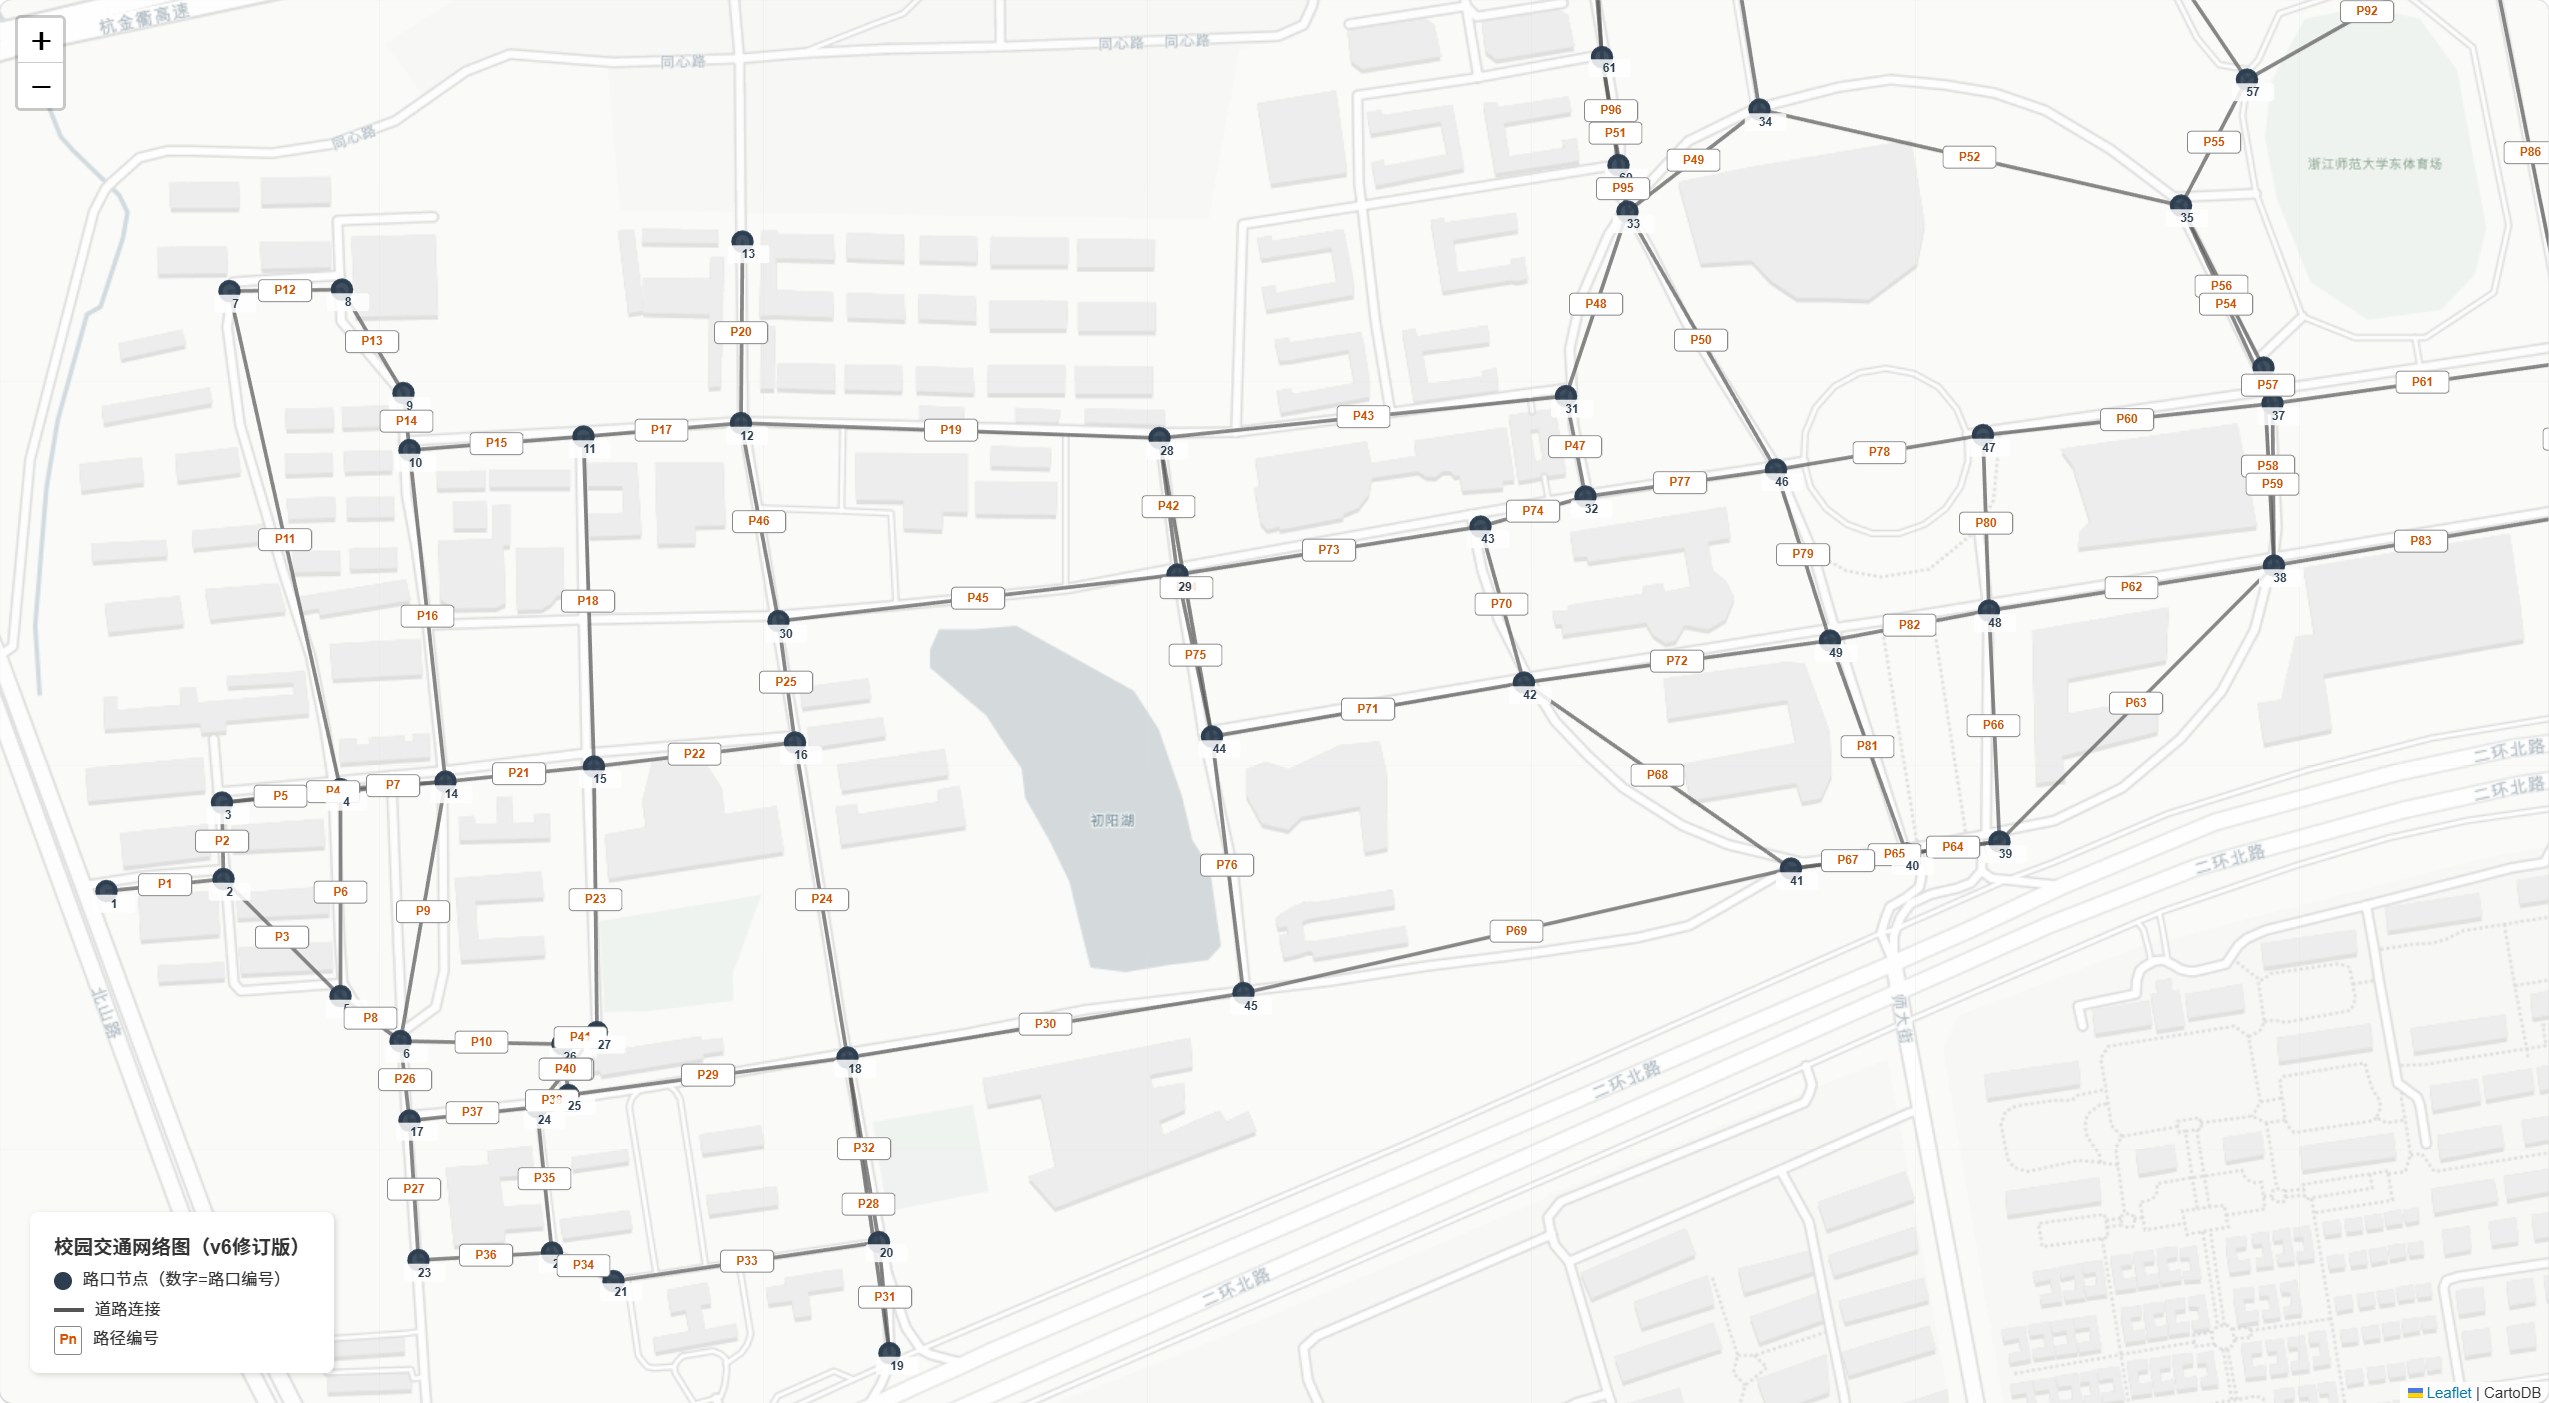
\includegraphics[width=0.65\linewidth]{figures/zjnu_map.png}
\caption{浙师大校园交通网络图，含84个节点、310条有向边}
\label{fig:campus_network}
\end{figure}

在本文路网模型中，建筑节点（宿舍、教学楼、食堂、商业街）并非直接坐落在道路上，而是作为交通发生/吸引的形心节点独立存在。每栋建筑通过 $2\sim5$ 条虚拟连接线挂载至周边最近的道路交叉口节点，形成辐条式接入结构。
由于缺少逐OD实测数据，本文采用引力模型估计高峰期出行分布$^{[1]}$。时段 $h$ 下，从建筑 $i$ 到建筑 $j$ 的出行需求为
\begin{equation}
T_{ij}^{h}=O_i^h\cdot \frac{D_j(d_{ij})^{-\gamma}}{\sum_kD_k(d_{ik})^{-\gamma}},
\end{equation}
其中 $O_i^h$ 为出发建筑在时段 $h$ 的出行产生量，$D_j$ 为到达建筑吸引力，$d_{ij}$ 为网络最短路径距离；考虑到校园封闭路网内师生对中长距离（如宿舍到食堂）出行敏感度的适中特性，距离衰减系数取 $\gamma=1.5$。

根据公开数据显示，全校本科生共计28,000左右，建筑容量与时段负荷系数作为OD生成参数（宿舍早0.90/教学楼午0.93/教学楼晚0.86）。

在得到 OD 总量后，按出行距离划分交通方式：短距离以步行为主，中长距离以电动车为主，远距离保留少量机动车需求。三时段 OD 估计结果见表\ref{tab:od_summary}。

\begin{table}[H]
\footnotesize
\centering
\caption{三时段OD需求估计结果}
\label{tab:od_summary}
\begin{tabular}{cccc}
\toprule
\textbf{时段} & \textbf{主要方向} & \textbf{OD总量/人次} & \textbf{电动车人次} \\
\midrule
早高峰 & 宿舍区 $\rightarrow$ 教学区 & 11,340 & 4,146 \\
午高峰 & 教学区 $\rightarrow$ 食堂/商业街 & 12,000 & 4,393 \\
晚高峰 & 教学区 $\rightarrow$ 宿舍/食堂 & 12,900 & 4,542 \\
\bottomrule
\end{tabular}
\end{table}

\subsubsection{多方式用户均衡分配模型}

为统一刻画步行、电动车和机动车的混行影响，将三类方式转换为等效PCU流量：
\begin{equation}
X_e^h=\sum_{m\in M}\xi_m x_e^{m,h},\qquad M=\{p,b,c\},
\end{equation}
其中 $p,b,c$ 分别表示步行、电动车和机动车，$x_e^{m,h}$ 为方式 $m$ 在路段 $e$、时段 $h$ 的流量，$\xi_m$ 为等效换算系数。路段阻抗采用BPR函数：
\begin{equation}
t_e^h=t_e^0\left[1+\alpha\left(\frac{X_e^h}{C_e}\right)^\beta\right],
\end{equation}
其中 $t_e^0=l_e/v_e^0$。在缺乏大规模实测校准数据的情况下，阻抗参数参考美国联邦公路局（FHWA）标准BPR函数推荐值$^{[2]}$，取 $\alpha=0.15$，$\beta=4.0$，以较好地刻画流量逼近通行能力时拥堵的急剧恶化现象。

用户均衡假设为：同一OD对、同一交通方式下，被选择路径的出行阻抗相等且不大于未被选择路径$^{[3]}$。对应的Beckmann等价规划为
\begin{equation}
\begin{aligned}
\min \quad & Z=\sum_{e\in E}\int_0^{X_e^h}t_e(w)\,dw,\\
\text{s.t.}\quad & \sum_{k\in K_{ij}} f_{k,ij}^{m,h}=q_{ij}^{m,h},\quad \forall(i,j),m,h,\\
& x_e^{m,h}=\sum_{(i,j)}\sum_{k\in K_{ij}}\delta_{e,k}^{ij}f_{k,ij}^{m,h},\quad \forall e,m,h,\\
& f_{k,ij}^{m,h}\ge 0.
\end{aligned}
\end{equation}
采用Frank--Wolfe算法求解$^{[4]}$。每轮迭代执行全有全无分配获得下降方向，一维线搜索确定步长，至收敛条件满足。

\subsubsection{微观精细化路径分流模型}

在上述宏观用户均衡（UE）分配模型的基础上，为进一步解决特定核心楼宇（如16号楼、25号楼）出入导致的微观流线交织问题，本文在此建立MinMax V/C增量分配模型。模型核心思想是将各时段OD需求按$B=60$个小批次等量切分，利用动态阻抗将车流“自适应铺摊”到低负荷路径上。

具体地，微观路段$e$在第$b$批分配时的动态阻抗定义为
\begin{equation}
t_e^b(m)=t_e^{0}(m)\cdot\Bigl[1+\lambda\cdot\bigl(\frac{X_e^{b-1}}{C_e}\bigr)^{\beta_p}+\eta\cdot\max\bigl(0,\frac{X_e^{b-1}}{C_e}-0.75\bigr)^2+\gamma\cdot\max(0,\frac{8-w_e}{8})\Bigr],
\end{equation}
其中$\lambda=65$、$\beta_p=4$控制拥堵惩罚强度（经网格测试标定，既能消除路段“拥死”也能避免过度绕行）；$\eta=140$作为高敏感系数，对$V/C>0.75$的高危过饱和路段施加额外超容惩罚；$\gamma=0.4$对窄路（宽度$<8$m）施加通行折扣以模拟窄路在混行条件下的通行能力剥减。对于特定楼宇的定向疏导，三方式（步行、电动车、机动车）将分别依此阻抗独立进行增量Dijkstra最短路径搜索。

\subsubsection{评价指标与现状基准分析}

结合上述模型算法，首先制定量化评价指标。模型评价指标包括总行程时间、冲突风险和道路饱和度。总行程时间定义为
\begin{equation}
TTT=\sum_{h\in\mathcal{H}}\sum_{e\in E}\sum_{m\in M}x_e^{m,h}t_e^h.
\end{equation}
人车冲突风险定义为不同方式流量乘积的加权和：
\begin{equation}
S_e^h=\omega_{pb}x_e^{p,h}x_e^{b,h}+\omega_{pc}x_e^{p,h}x_e^{c,h}+\omega_{bc}x_e^{b,h}x_e^{c,h},
\end{equation}
其中风险权重系数根据不同交通工具的质量差和速度差决定：机动车与行人混行的伤害严重程度最大（设定 $\omega_{pc}=1.5$），机动车与电动车次之（设定 $\omega_{bc}=0.8$），电动车与行人的相对质量差小，伤害风险相对较低（设定 $\omega_{pb}=0.5$）。全路网风险为 $S=\sum_{h,e}S_e^h$。道路饱和度为 $\mu_e^h=X_e^h/C_e$，用于识别宏观层面的瓶颈路段。

在不采取治理措施的基准情景下，三个时段分别进行用户均衡分配，结果如表\ref{tab:baseline}所示。午高峰TTT和$S$均为三时段最高，原因是12栋教学楼同时向食堂和商业街方向集中释放出行需求，多方向流线在网络中叠加，冲突风险显著高于早、晚的单向通勤流。

\begin{table}[H]
\footnotesize
\centering
\caption{现状情景三时段UE分配结果}
\label{tab:baseline}
\begin{tabular}{cccc}
\toprule
\textbf{时段} & \textbf{TTT} & \textbf{冲突风险 $S$} & \textbf{核心瓶颈路段} \\
\midrule
早高峰 & 2,557,530 & 7,651,286 & $N4\rightarrow N14$，V/C=1.249 \\
午高峰 & 2,980,097 & 11,419,251 & $N16\rightarrow N30$，V/C=1.410 \\
晚高峰 & 2,490,034 & 7,636,591 & $N14\rightarrow N4$，V/C=1.251 \\
\midrule
合计 & 8,027,661 & 26,707,128 & --- \\
\bottomrule
\end{tabular}
\end{table}

\subsubsection{宏观交通组织方案设计与安全评价}

针对现状瓶颈和冲突风险分布，从路网结构层面设计三类方案进行比选。方案A在早高峰关键路段设置单行线（N30$\to$N16、N4$\to$N14、N49$\to$N48）；方案B在午高峰对N16$\to$N30、N48$\to$N49等11条高V/C路段降容60\%并削减机动车需求至30\%；方案C为方案C，将方案A、方案B与高风险路段人车隔离合并，对冲突风险最高的18条路段设置物理隔离。

三类方案的效果比较见表\ref{tab:scenario_compare}（$\Delta TTT$ 负值表示总行程时间增加，$\Delta S$ 正值表示安全水平改善）：

\begin{table}[H]
\footnotesize
\centering
\caption{三类治理方案效果对比}
\label{tab:scenario_compare}
\begin{tabular}{ccccc}
\toprule
\textbf{方案} & \textbf{TTT} & \textbf{$\Delta TTT$} & \textbf{冲突风险 $S$} & \textbf{$\Delta S$} \\
\midrule
基准现状 & 7,949,785 & --- & 28,963,236 & --- \\
方案A：单行线 & 8,120,949 & $-1.1\%$ & 27,403,631 & $+5.4\%$ \\
方案B：限行+削减 & 8,118,808 & $-1.0\%$ & 24,903,939 & $+14.0\%$ \\
\textbf{方案C} & 8,223,148 & $-2.2\%$ & \textbf{22,030,958} & \textbf{$+25.3\%$} \\
\bottomrule
\end{tabular}
\end{table}

方案C的$\Delta S=25.3\%$，高于方案A（5.4\%）和方案B（14.0\%）。$\Delta TTT=-2.2\%$，增量来自单行线和限行造成的绕行。

\begin{figure}[H]
\centering
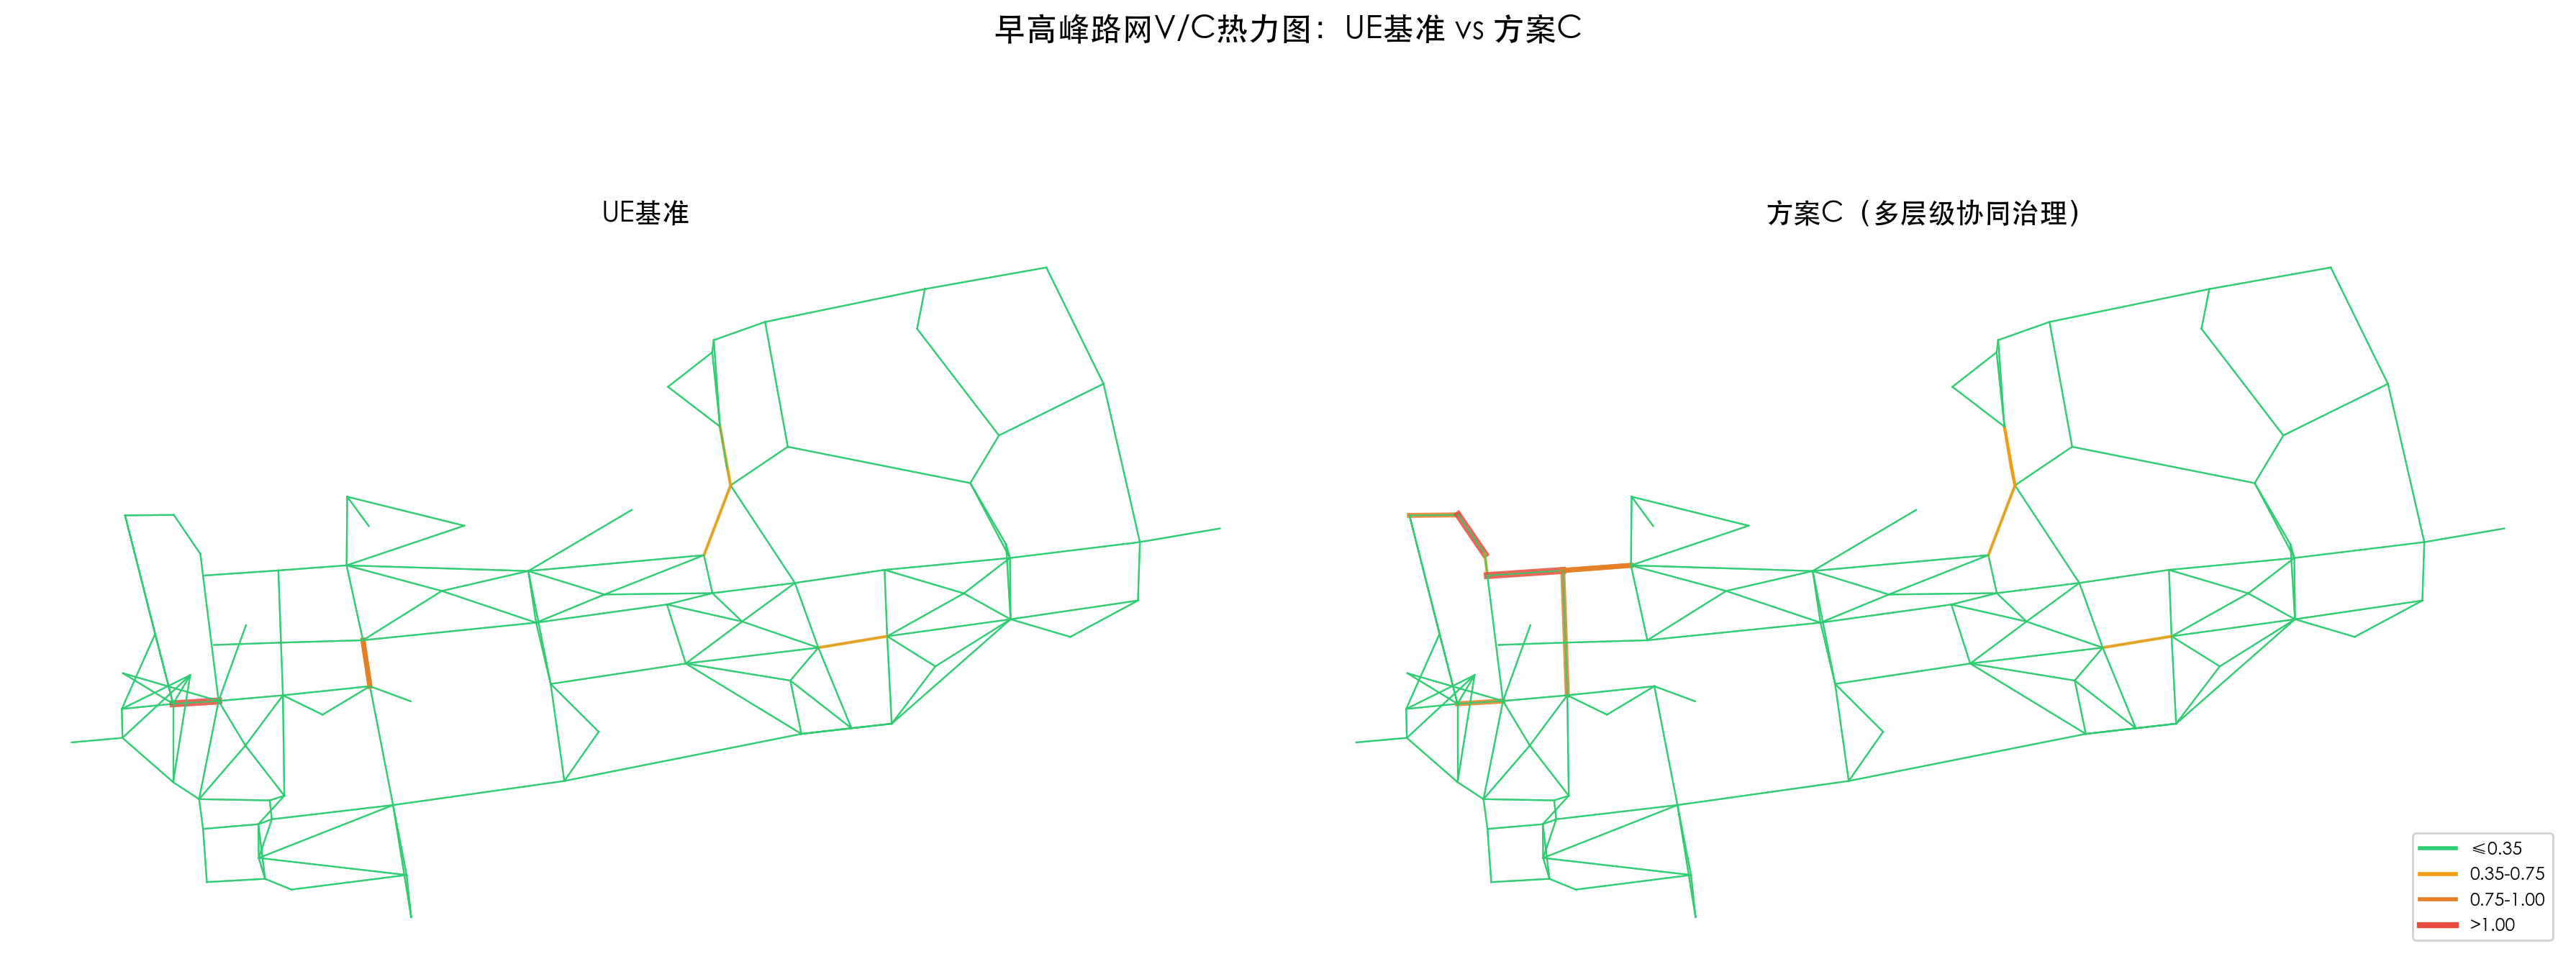
\includegraphics[width=0.65\linewidth]{figures/heatmap_morning_schemeC.png}
\caption{早高峰路网V/C热力图（左：UE基准，右：方案C改造后）}
\label{fig:heatmap_schemeC}
\end{figure}

图\ref{fig:heatmap_schemeC}显示，方案C将N4$\to$N14路段V/C从1.249降至1.053，但造成负面转移：N8$\to$N9与N10$\to$N11路段骤升至1.053，全路网过饱和路段从1条增至2条。方案C以降低冲突风险换取路网效率，但绕行诱发了新的拥堵点，难以兼顾安全与效率。

\subsubsection{微观分流效果评估与最优路径生成}\label{sec:minmax}

上述宏观方案从路网结构层面降低了冲突风险，但存在两个局限：一是物理改造（如单行线）会强制绕行，可能诱发新的拥堵点；二是UE分配中所有出行者仍选择单一最短路径，导致瓶颈路段流量集中。为此，本节在不改动路网结构的条件下，建立MinMax V/C增量分配模型，通过动态路径引导实现车流的"自适应铺摊"。

模型将各时段OD需求按$B=60$批次依次释放，每批次根据当前饱和度更新阻抗，使后续车流自动避开已拥堵路段。三时段最大V/C变化如表\ref{tab:minmax_result}所示：

\begin{figure}[H]
\centering

\includegraphics[width=0.65\linewidth]{figures/heatmap_morning.png}
\caption{早高峰路网V/C热力图（左：UE基准，右：MinMax增量分配优化）}
\label{fig:heatmap_morning}
\end{figure}

图\ref{fig:heatmap_morning}显示，MinMax优化后N4$\to$N14路段V/C从1.249降至0.255（降幅79.6\%），过饱和路段清零。

\begin{table}[H]
\footnotesize
\centering
\caption{MinMax V/C微观增量分配优化效果}
\label{tab:minmax_result}
\begin{tabular}{cccc}
\toprule
\textbf{时段} & \textbf{基准max V/C} & \textbf{微观优化后max V/C} & \textbf{降幅} \\
\midrule
早高峰 & 1.249 & 0.255 & 79.6\% \\
午高峰 & 1.410 & 0.469 & 66.7\% \\
晚高峰 & 1.251 & 0.700 & 44.1\% \\
\bottomrule
\end{tabular}
\end{table}

优化后全路网无V/C>1.00的过饱和路段。MinMax输出包括每对OD在各方式下的具体分流路径。以早高峰TYGY至T\_16的电动车出行为例，算法生成两条路径：

\begin{itemize}
  \item \textbf{直达路径}（35人）：TYGY $\to$ N4 $\to$ N14 $\to$ T\_2 $\to$ N15 $\to$ T\_16，全程较短但需穿过 N4$\to$N14 窄路段（宽6m）；
  \item \textbf{绕行路径}（228人）：TYGY $\to$ N4 $\to$ T\_4 $\to$ N14 $\to$ T\_2 $\to$ N15 $\to$ T\_16，经 T\_4 绕行避开拥挤段。
\end{itemize}

86.7\%的电动车流量被分配至绕行路径。全路网2284条路径记录覆盖了所有关键OD对，可作为导流标识设置的数据基础。

\textbf{方案对比与结论：}综合对比方案C（路网结构改造）与MinMax增量分流（路径分配优化）的效果：方案C虽能降低冲突风险25.3\%，但绕行诱发了新的拥堵点，过饱和路段从1条增至2条；而MinMax方案在不改动路网的条件下，将最大V/C从1.249降至0.255，过饱和路段清零，且无任何路段恶化。因此，问题一的交通流优化最终采用MinMax方案作为核心优化手段，方案C的路网结构改造（单行线、人车隔离等）作为辅助治理建议，在问题四中进一步讨论。

\newpage

\section{电动车承载力评估}

\subsection{问题重述}

校园电动车数量持续增长，教学楼、宿舍区、食堂和商业街周边出现停车紧张、乱停放和通行干扰。
问题二要求在不占用消防通道的前提下，结合道路宽度和建筑周边停车面积，测算校园可承载的最大电动车数量。
结果将作为学校后续总量控制、分区停放和停车治理的依据。

\subsection{问题分析}

问题二采用“静态停车容量+动态道路容量+消防折减”的三层校核思路：先算建筑周边可停面积，再算道路接入能力，最后取两者较小值作为安全承载力。
通过分区测算可以识别哪里是停车瓶颈、哪里是道路瓶颈，从而给出校园电动车总量控制上限。

\subsection{模型假设}

作如下假设：
\begin{enumerate}
    \item 电动车停放限于建筑周边可规划区域，不占用消防通道、出入口、主通行人行道和绿化隔离带；
    \item 每辆两轮电动车的基本占地面积取 $a_e=1.08\,\text{m}^2$，并通过停车间距和通道系数 $\beta$ 反映实际规范停放所需附加空间；
    \item 各区域停车面积在短期内不发生结构性变化，安全折减系数可反映消防通道、疏散空间和不可停车空间的综合影响；
    \item 动态道路容量由区域周边可接入道路的通行能力决定，并与问题一中得到的路网容量和高峰运行状态保持一致；
    \item 校园电动车治理应同时区分高峰运行需求和车辆实际保有量，前者用于高峰运行校核，后者用于存量总量管理校核。
\end{enumerate}

\subsection{符号说明}

\begin{table}[H]
\footnotesize
\centering
\caption{问题二主要符号说明}
\label{tab:symbols_q2}
\begin{tabular}{ccc}
\toprule
\textbf{符号} & \textbf{说明} & \textbf{单位} \\
\midrule
$A_i^{raw}$ & 区域 $i$ 原始候选停车面积 & $\text{m}^2$ \\
$\lambda_i$ & 区域 $i$ 的消防安全折减系数 & -- \\
$A_i^{eff}$ & 区域 $i$ 有效停车面积 & $\text{m}^2$ \\
$a_e$ & 单辆电动车基本占地面积 & $\text{m}^2$/辆 \\
$\beta$ & 规范停放附加空间系数 & -- \\
$N_i^{static}$ & 区域 $i$ 静态停车容量 & 辆 \\
$N_i^{dynamic}$ & 区域 $i$ 动态道路容量 & 辆 \\
$N_i^*$ & 区域 $i$ 最终安全承载力 & 辆 \\
$N_{max}$ & 全校电动车安全环境承载力 & 辆 \\
$D_i^{peak}$ & 区域 $i$ 高峰停车或运行需求 & 辆 \\
$\rho_i$ & 区域 $i$ 饱和度 & -- \\
\bottomrule
\end{tabular}
\end{table}

\subsection{模型的建立与求解}

\subsubsection{静态停车容量模型}

根据《建筑设计防火规范》（GB\,50016）对消防车道净宽度的强制性要求$^{[5]}$，原始候选面积不能全部用于停车，需要严格扣除消防通道、建筑出入口、主通行人行道、绿化隔离带和必要疏散空间。为此，引入区域安全折减系数 $\lambda_i$，得到有效停车面积：
\begin{equation}
A_i^{eff}=\lambda_i A_i^{raw}.
\end{equation}
其中，$0<\lambda_i<1$。生活区和商业街人流密度较高、消防疏散要求更严格，折减系数相对较小；教学区周边若有较明确的开敞空间，折减系数可略高。

设单辆电动车基本占地面积为 $a_e$，规范停放附加空间系数为 $\beta$，则区域 $i$ 的静态停车容量为
\begin{equation}
N_i^{static}=\left\lfloor \frac{A_i^{eff}}{\beta a_e}\right\rfloor .
\end{equation}
考虑到常规两轮电动车的物理尺寸及《城市非机动车交通系统规划设计导则》的相关规定$^{[6]}$，取其基本物理占地面积为 $a_e=1.08\,\text{m}^2$；同时为保证车辆独立进出互不干扰，参考规范停放标准，附加空间系数取 $\beta=1.35$，以计入必要的停车间隔、通行缝隙和实际管理中的无效冗余。

\begin{table}[H]
\footnotesize
\centering
\caption{消防安全折减后的静态容量测算结果}
\label{tab:static_capacity}
\begin{tabular}{ccccc}
\toprule
\textbf{区域} & \textbf{原始面积/m$^2$} & \textbf{折减系数} & \textbf{有效面积/m$^2$} & \textbf{静态容量/辆} \\
\midrule
16号楼教学区 & 630 & 0.72 & 450 & 308 \\
25号楼教学区 & 770 & 0.72 & 550 & 377 \\
桃源生活区 & 13000 & 0.63 & 8160 & 5596 \\
杏园生活区 & 7800 & 0.65 & 5100 & 3497 \\
桂苑生活区 & 12000 & 0.63 & 7700 & 5281 \\
东区新教学楼 & 3200 & 0.70 & 2200 & 1508 \\
西区新教学楼 & 5700 & 0.70 & 4000 & 2743 \\
商业街 & 1900 & 0.60 & 1200 & 823 \\
\bottomrule
\end{tabular}
\end{table}

\subsubsection{动态道路容量模型}

静态停车容量反映停放能力，动态道路容量反映周边道路接入能力。区域 $i$ 的接入路段集合为 $E_i$，路段 $e$ 通行能力为 $C_e$，电动车可分配比例为 $\eta_b$，高峰持续时间 $T_h$，动态道路容量为
\begin{equation}
N_i^{dynamic}=\sum_{e\in E_i}\eta_b C_e T_h.
\end{equation}
该容量与问题一中路网参数和高峰运行状态衔接。

\subsubsection{综合承载力模型}

区域最终承载力由静态停车容量和动态道路容量共同约束，取二者较小值：
\begin{equation}
N_i^*=\min\left(N_i^{static},N_i^{dynamic}\right).
\end{equation}
全校电动车安全环境承载力为各区域承载力之和：
\begin{equation}
N_{max}=\sum_i N_i^*.
\end{equation}
区域饱和度定义为
\begin{equation}
\rho_i=\frac{D_i^{peak}}{N_i^*},
\end{equation}
其中 $D_i^{peak}$ 为区域高峰需求。$\rho_i>1$ 表示超载，$\rho_i\approx1$ 表示饱和，$\rho_i<1$ 表示容量充足。

\begin{table}[H]
\footnotesize
\centering
\caption{区域综合承载力与高峰需求校核结果}
\label{tab:capacity_result}
\begin{tabular}{cccccc}
\toprule
\textbf{区域} & \textbf{$N^{static}$} & \textbf{$N^{dynamic}$} & \textbf{$N^*$} & \textbf{$D_i$} & \textbf{$\rho$} \\
\midrule
16号楼教学区 & 308 & 1482 & 308 & 689 & 2.235 \\
25号楼教学区 & 377 & 1888 & 377 & 783 & 2.077 \\
桃园生活区 & 5596 & 1888 & 1888 & 2334 & 1.237 \\
杏园生活区 & 3497 & 1370 & 1370 & 1129 & 0.824 \\
桂苑生活区 & 5281 & 709 & 709 & 1221 & 1.722 \\
东区新教学楼 & 1508 & 1482 & 1482 & 311 & 0.210 \\
西区新教学楼 & 2743 & 1793 & 1793 & 415 & 0.232 \\
商业街 & 823 & 1482 & 823 & 2101 & 2.553 \\
\bottomrule
\end{tabular}
\end{table}

由表\ref{tab:capacity_result}，16号楼、25号楼、商业街和桂苑生活区四个区域超载（而非道路通行能力不足），桃园、杏园、桂苑生活区受动态道路容量约束。

\begin{figure}[H]
\centering
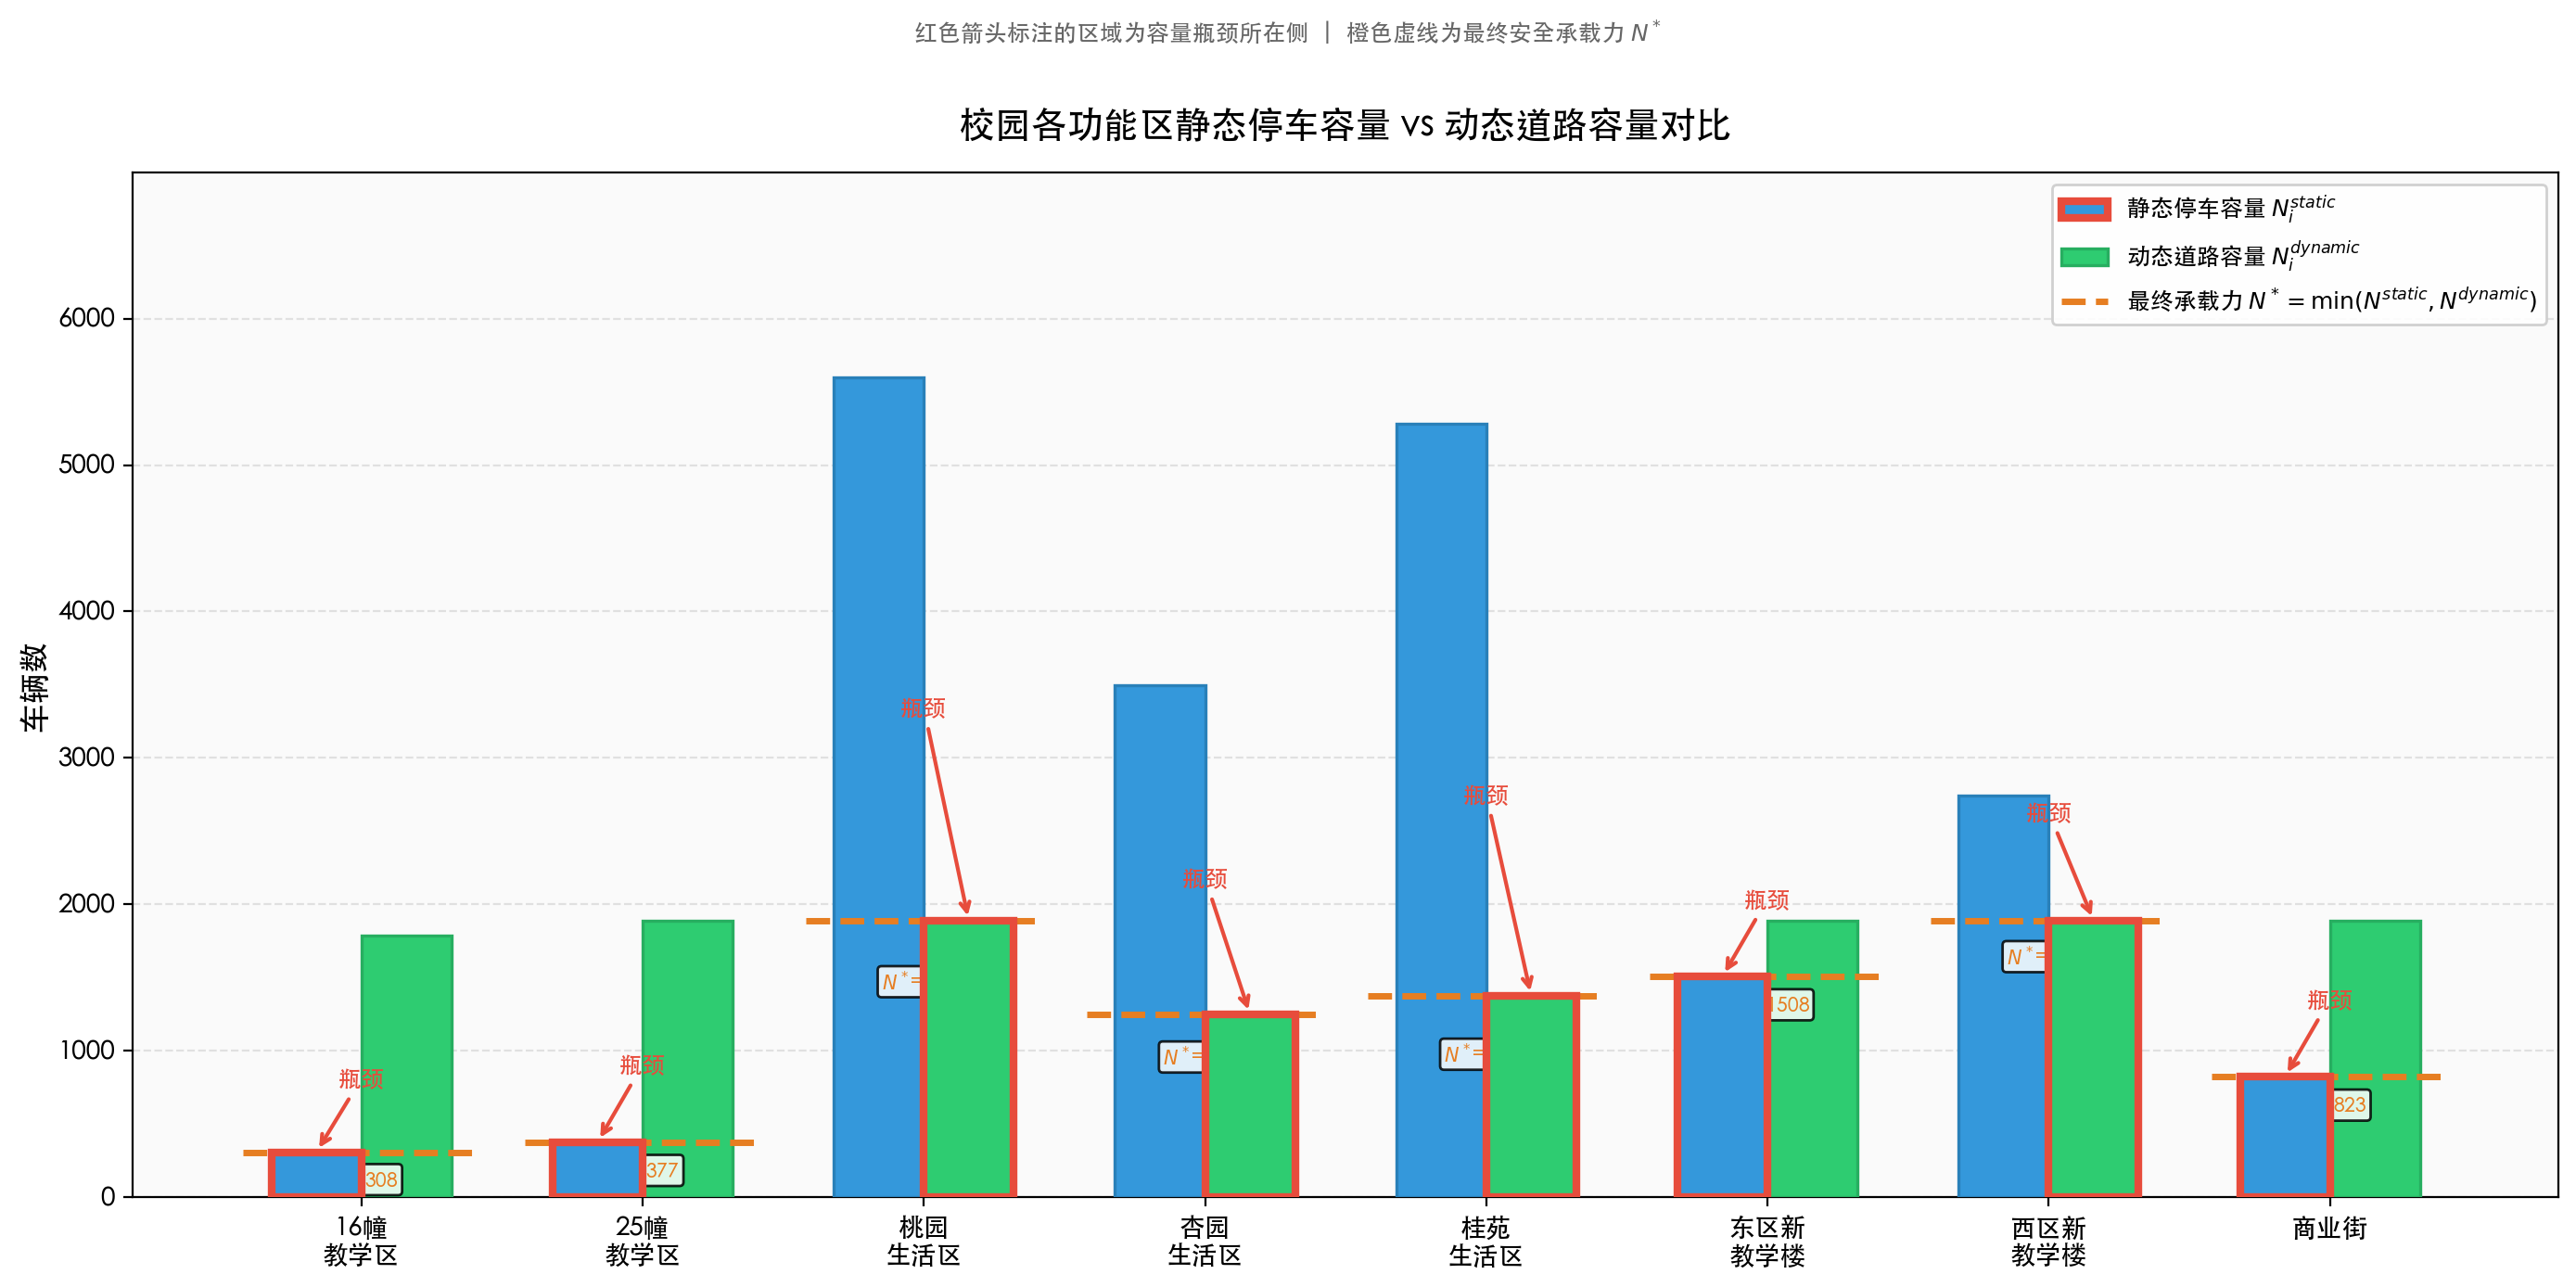
\includegraphics[width=0.65\linewidth]{figures/static_vs_dynamic.png}
\caption{各功能区静态停车容量与动态道路容量对比}
\label{fig:static_vs_dynamic}
\end{figure}

\subsubsection{全校承载力与双层饱和度校核}

将各区域最终容量汇总，得到全校电动车安全环境承载力为
\begin{equation}
N_{max}=9414\text{ 辆}.
\end{equation}
如果仅以模型估计的最差时段高峰运行需求进行校核，最大电动车运行需求为5166辆，则高峰运行饱和度为
\begin{equation}
\theta_{peak}=\frac{5166}{9414}=0.549.
\end{equation}
在OD模型口径下，高峰时段进入道路和停车系统的电动车规模未超过全校安全承载力。

高峰运行需求不等同于实际保有量。按公开资料中11000辆以上保有量校核：
\begin{equation}
\theta_{stock}=\frac{11000}{9414}\approx 1.168,
\end{equation}
\begin{equation}
11000-9414=1586\text{ 辆}.
\end{equation}
\textbf{按高峰OD需求校核，运行量未超过安全承载力；按实际保有量校核，存量已明显超过安全承载力。}

\subsubsection{敏感性检验：有效面积测量误差}

承载力对区域有效停车面积 $A_i^{eff}$ 的测量精度存在依赖。但需要注意，各区域的最终承载力 $N_i^*=\min(N_i^{static},N_i^{dynamic})$ 由静态和动态容量中的较小者决定——在8个区域中，仅16号楼教学区、25号楼教学区和商业街3个区域受静态面积约束，其余5个区域（桃园、杏园、桂苑、东区、西区）均受动态道路容量约束。因此，$A_i^{eff}$ 的扰动并不会线性传导至 $N_{max}$。

为检验结论稳健性，对 $A_i^{eff}$ 施加 $\pm20\%$ 均匀扰动，重新计算各区域 $N_i^{static}$ 并与 $N_i^{dynamic}$ 取较小值，结果如表\ref{tab:sensitivity_area}所示。

\begin{table}[H]
\footnotesize
\centering
\caption{N\_max 对有效停车面积测量误差的敏感性}
\label{tab:sensitivity_area}
\begin{tabular}{cccc}
\toprule
\textbf{扰动幅度} & \textbf{$N_{max}$（辆）} & \textbf{$\Delta N_{max}$} & \textbf{$\theta_{peak}$} \\
\midrule
$-20\%$（低估） & 8809 & $-6.4\%$ & 0.586 \\
$-10\%$ & 9111 & $-3.2\%$ & 0.567 \\
基准（0\%） & 9414 & -- & 0.549 \\
$+10\%$ & 9713 & $+3.2\%$ & 0.532 \\
$+20\%$（高估） & 10015 & $+6.4\%$ & 0.516 \\
\bottomrule
\end{tabular}
\end{table}

结果表明，当 $A_i^{eff}$ 扰动 $\pm20\%$ 时，承载力变化仅约 $\pm6.4\%$，且高峰运行饱和度 $\theta_{peak}$ 仍$<1$。结论极具稳健性，不会改变“运行未超载、存量已超载”的定性结果。

\subsubsection{问题二结论与治理建议}

综合校核得出：（1）金华校区电动车安全承载力约9414辆；（2）高峰运行无整体拥堵（饱和度0.549），但存量超载达1.168；（3）空间失衡严重，16/25号楼及商业街极度拥挤。治理建议实施“存量绝对控制+核心区禁停+外围缓冲限流”。

\newpage

\section{微公交选址与调度}

\subsection{问题重述}

为减少师生对私人电动车的依赖，学校计划投放校园微公交，缓解教学区、宿舍区、食堂和商业街之间的高峰出行压力。
问题三要求基于校园空间拓扑确定接驳线路和站点，保证覆盖率的同时尽量不影响主干道通行。
同时结合潮汐客流确定车辆投放量和发车时间表，在满足需求的前提下降低运营成本。

\subsection{问题分析}

问题三分别用最大覆盖选址模型确定站点，用路径规划模型确定行驶线路，用车辆调度模型确定投放量和发车间隔。
其中站点选择强调覆盖需求和停靠安全，线路选择强调避开拥堵路段，调度部分则以最小化运营成本和等待成本为目标。

\subsection{模型假设}

作如下假设：
\begin{enumerate}
    \item 接驳车主要服务校园内部短距离高峰出行，不考虑校外长距离客流；
    \item 候选站点设置在宿舍区、核心教学楼、食堂或商业街周边，且停靠位置应满足道路宽度和安全条件；
    \item 接驳车运行速度受道路拥堵影响，可用问题一中的BPR阻抗思想修正路段运行时间；
    \item 微公交对私人电动车的替代需求由基础替代需求决定；
    \item 接驳车按固定线路循环或往返运行，同一时段内车辆均匀发车，乘客平均等待时间约为发车间隔的一半；
    \item 调度目标是在满足客流需求和最大发车间隔约束下，使运营成本、乘客等待成本和运能浪费成本之和最小。
\end{enumerate}

\subsection{符号说明}

\begin{table}[H]
\footnotesize
\centering
\caption{问题三主要符号说明}
\label{tab:symbols_q3}
\begin{tabular}{ccc}
\toprule
\textbf{符号} & \textbf{说明} & \textbf{单位} \\
\midrule
$I$ & 需求点集合 & -- \\
$J$ & 候选站点集合 & -- \\
$x_j$ & 候选站点 $j$ 是否被选中 & 0--1 \\
$y_i$ & 需求点 $i$ 是否被覆盖 & 0--1 \\
$a_i$ & 需求点 $i$ 的需求权重 & 人次 \\
$r_{ij}$ & 站点 $j$ 是否覆盖需求点 $i$ & 0--1 \\
$P_j$ & 候选站点 $j$ 的适宜性得分 & -- \\
$D_s^t$ & 时段 $t$ 的接驳需求 & 人次 \\
$D_{bike}^t$ & 时段 $t$ 的电动车运行需求 & 人次 \\
$N_{max}$ & 校园电动车安全承载力 & 辆 \\
$n_t$ & 时段 $t$ 投放接驳车辆数 & 辆 \\
$K$ & 单车载客量 & 人/车 \\
$\tau_r$ & 推荐线路单程运行时间 & min \\
$h_t$ & 时段 $t$ 发车间隔 & min \\
\bottomrule
\end{tabular}
\end{table}

\subsection{模型的建立与求解}

\subsubsection{候选站点构造与适宜性评价}

根据校园空间结构和问题二中识别出的高压区域，选取宿舍区、16号楼、25号楼、食堂和商业街周边作为候选站点。设候选站点集合为 $J$，需求点集合为 $I$。候选站点是否适宜停靠，需要同时考虑覆盖能力、道路宽度、拥堵程度和冲突风险。站点 $j$ 对需求点 $i$ 的覆盖关系定义为
\begin{equation}
r_{ij}=\begin{cases}
1, & d_{ij}\le R_0,\\
0, & d_{ij}>R_0,
\end{cases}
\end{equation}
其中 $d_{ij}$ 为需求点 $i$ 到候选站点 $j$ 的步行距离，$R_0$ 为最大可接受步行距离。

进一步构造候选站点适宜性得分：
\begin{equation}
P_j=\alpha_1 COV_j+\alpha_2 W_j-\alpha_3 VC_j-\alpha_4 RISK_j,
\end{equation}
其中 $COV_j$ 表示站点覆盖需求强度，$W_j$ 表示周边道路宽度条件，$VC_j$ 表示周边道路饱和度，$RISK_j$ 表示周边冲突风险。适宜性得分越高，说明该站点既能覆盖更多需求，又不容易因停靠造成额外拥堵或安全风险。

\subsubsection{最大覆盖站点选址模型}

在候选站点适宜性评价基础上，建立最大覆盖选址模型$^{[7]}$。设 $x_j$ 表示候选站点 $j$ 是否被选中，$y_i$ 表示需求点 $i$ 是否被覆盖，$p$ 为可建设站点数量，则模型为
\begin{equation}
\begin{aligned}
\max \quad & \sum_{i\in I} a_i y_i,\\
\text{s.t.}\quad & y_i\le \sum_{j\in J} r_{ij}x_j,\quad \forall i\in I,\\
& \sum_{j\in J}x_j=p,\\
& x_j\in\{0,1\},\quad y_i\in\{0,1\}.
\end{aligned}
\end{equation}
其中 $a_i$ 为需求点权重，可由建筑容量、高峰OD需求和停车压力综合确定。模型目标是在给定站点数量下最大化被覆盖需求。计算结果表明，选取桃源站、16号楼站、25号楼站、杏园站和桂苑站能够较好覆盖宿舍区与核心教学区之间的潮汐客流，并兼顾食堂和生活区方向的出行需求。

\subsubsection{基于BPR阻抗的线路规划模型}

接驳车运行线路以BPR阻抗修正的通行时间为边权进行最短路搜索。沿用问题一中的BPR阻抗：
\begin{equation}
t_e^{bus}=\frac{l_e}{v_{bus}}\left[1+\alpha\left(\frac{X_e}{C_e}\right)^\beta\right],
\end{equation}
其中 $v_{bus}$ 为接驳车自由流速度，$X_e/C_e$ 为路段饱和度；阻抗参数同样沿用 $\alpha=0.15$，$\beta=4.0$ 以保持路网整体阻抗计算的一致性。

为综合比较不同线路，构造线路广义成本函数：
\begin{equation}
G_r=\omega_1\frac{L_r}{L_{max}}+\omega_2\frac{T_r}{T_{max}}+\omega_3\overline{VC}_r+\omega_4\overline{RISK}_r-\omega_5\frac{Q_r}{Q_{max}},
\end{equation}
其中 $L_r$ 为线路长度，$T_r$ 为线路运行时间，$\overline{VC}_r$ 为线路平均饱和度，$\overline{RISK}_r$ 为线路平均冲突风险，$Q_r$ 为线路覆盖需求。广义成本越小，线路综合表现越优。

候选线路评价结果如表\ref{tab:route_eval}所示。R1教学潮汐线长度和运行时间较短，广义成本最低，因此选为推荐线路。

\begin{table}[H]
\footnotesize
\centering
\caption{候选接驳线路评价结果}
\label{tab:route_eval}
\begin{tabular}{ccccccc}
\toprule
\textbf{线路} & \textbf{类型} & \textbf{长度/m} & \textbf{时间/min} & \textbf{平均V/C} & \textbf{覆盖需求} & \textbf{广义成本} \\
\midrule
R1 & 教学潮汐线 & 1243 & 5.8 & 0.149 & 51,300 & 0.4352 \\
R2 & 校园环线 & 1661 & 7.9 & 0.180 & 51,300 & 0.6324 \\
\bottomrule
\end{tabular}
\end{table}

推荐线路为
\begin{equation}
\text{桃源站}\rightarrow\text{16号楼站}\rightarrow\text{25号楼站}\rightarrow\text{杏园站}\rightarrow\text{桂苑站}.
\end{equation}
该线路能够连接主要宿舍区和核心教学区，适合承担早高峰宿舍到教学楼、午高峰教学楼到食堂及生活区、晚高峰教学楼返回宿舍的潮汐出行需求。

\subsubsection{接驳需求识别模型}

本文将时段 $t$ 的接驳需求定义为
\begin{equation}
D_s^t=\eta_{base}D_{bike}^t,
\end{equation}
其中 $\eta_{base}$ 为基础绿色替代率。参考《2023年中国主要城市通勤监测报告》中关于常规微循环公共交通体系对个体的分担率$^{[8]}$，结合校园接驳车的发车频次与舒适度预期，基准情景取 $\eta_{base}=10\%$。由此得到早高峰、午高峰和晚高峰接驳需求分别为447、517和454人次。

\subsubsection{潮汐客流调度模型}

接驳车调度需要在满足客流需求的同时控制运营成本。设时段 $t$ 持续时间为 $H_t$，推荐线路单程运行时间为 $\tau_r$，投放车辆数为 $n_t$。单车容量 $K$ 取 25 人/车——参照现实校园接驳场景，中型客车在座位（约 15 座）基础上允许少量站立，实际容纳约 25 人，且车宽不足 2.5 m，可在校园最窄支路（宽 6 m）上正常通行。则发车间隔为
\begin{equation}
h_t=\frac{\tau_r}{n_t},
\end{equation}
时段总运能为
\begin{equation}
Q_t(n_t)=n_tK\frac{H_t}{\tau_r}.
\end{equation}

综合考虑车辆运营成本、乘客等待成本和运能浪费成本，建立调度成本函数：
\begin{equation}
Z(n_t)=C_Vn_tH_t+C_WD_s^t\frac{h_t}{2}+C_O\max(0,Q_t(n_t)-D_s^t),
\end{equation}
约束条件为
\begin{equation}
Q_t(n_t)\ge D_s^t,\qquad h_t\le H_{max},\qquad n_t\in \mathbb{Z}^{+}.
\end{equation}
其中第一项为车辆运营成本，第二项为乘客平均等待成本，第三项为运能闲置惩罚。通过枚举可行车辆数，选择总成本最小的 $n_t$ 作为推荐投放量。

\begin{table}[H]
\footnotesize
\centering
\caption{基准情景下接驳车调度结果}
\label{tab:dispatch_result}
\resizebox{\linewidth}{!}{
\begin{tabular}{cccccccc}
\toprule
\textbf{时段} & \textbf{主方向} & \textbf{需求/人次} & \textbf{持续/min} & \textbf{单程/min} & \textbf{车辆数} & \textbf{间隔/min} & \textbf{满载率} \\
\midrule
早高峰 & 宿舍区$\rightarrow$教学区 & 447 & 45 & 5.8 & 3 & 1.9 & 0.77 \\
午高峰 & 教学区$\rightarrow$食堂/商业街 & 517 & 50 & 5.8 & 3 & 1.9 & 0.80 \\
晚高峰 & 教学区$\rightarrow$宿舍/食堂 & 454 & 40 & 5.8 & 3 & 1.9 & 0.88 \\
\bottomrule
\end{tabular}
}
\end{table}

由表\ref{tab:dispatch_result}可知，基准10\%替代率下，三个时段各需投放3辆接驳车。各时段发车间隔均为1.9分钟，平均等待时间约1.0分钟，能够满足高峰期连续接驳需求。

\begin{figure}[H]
\centering
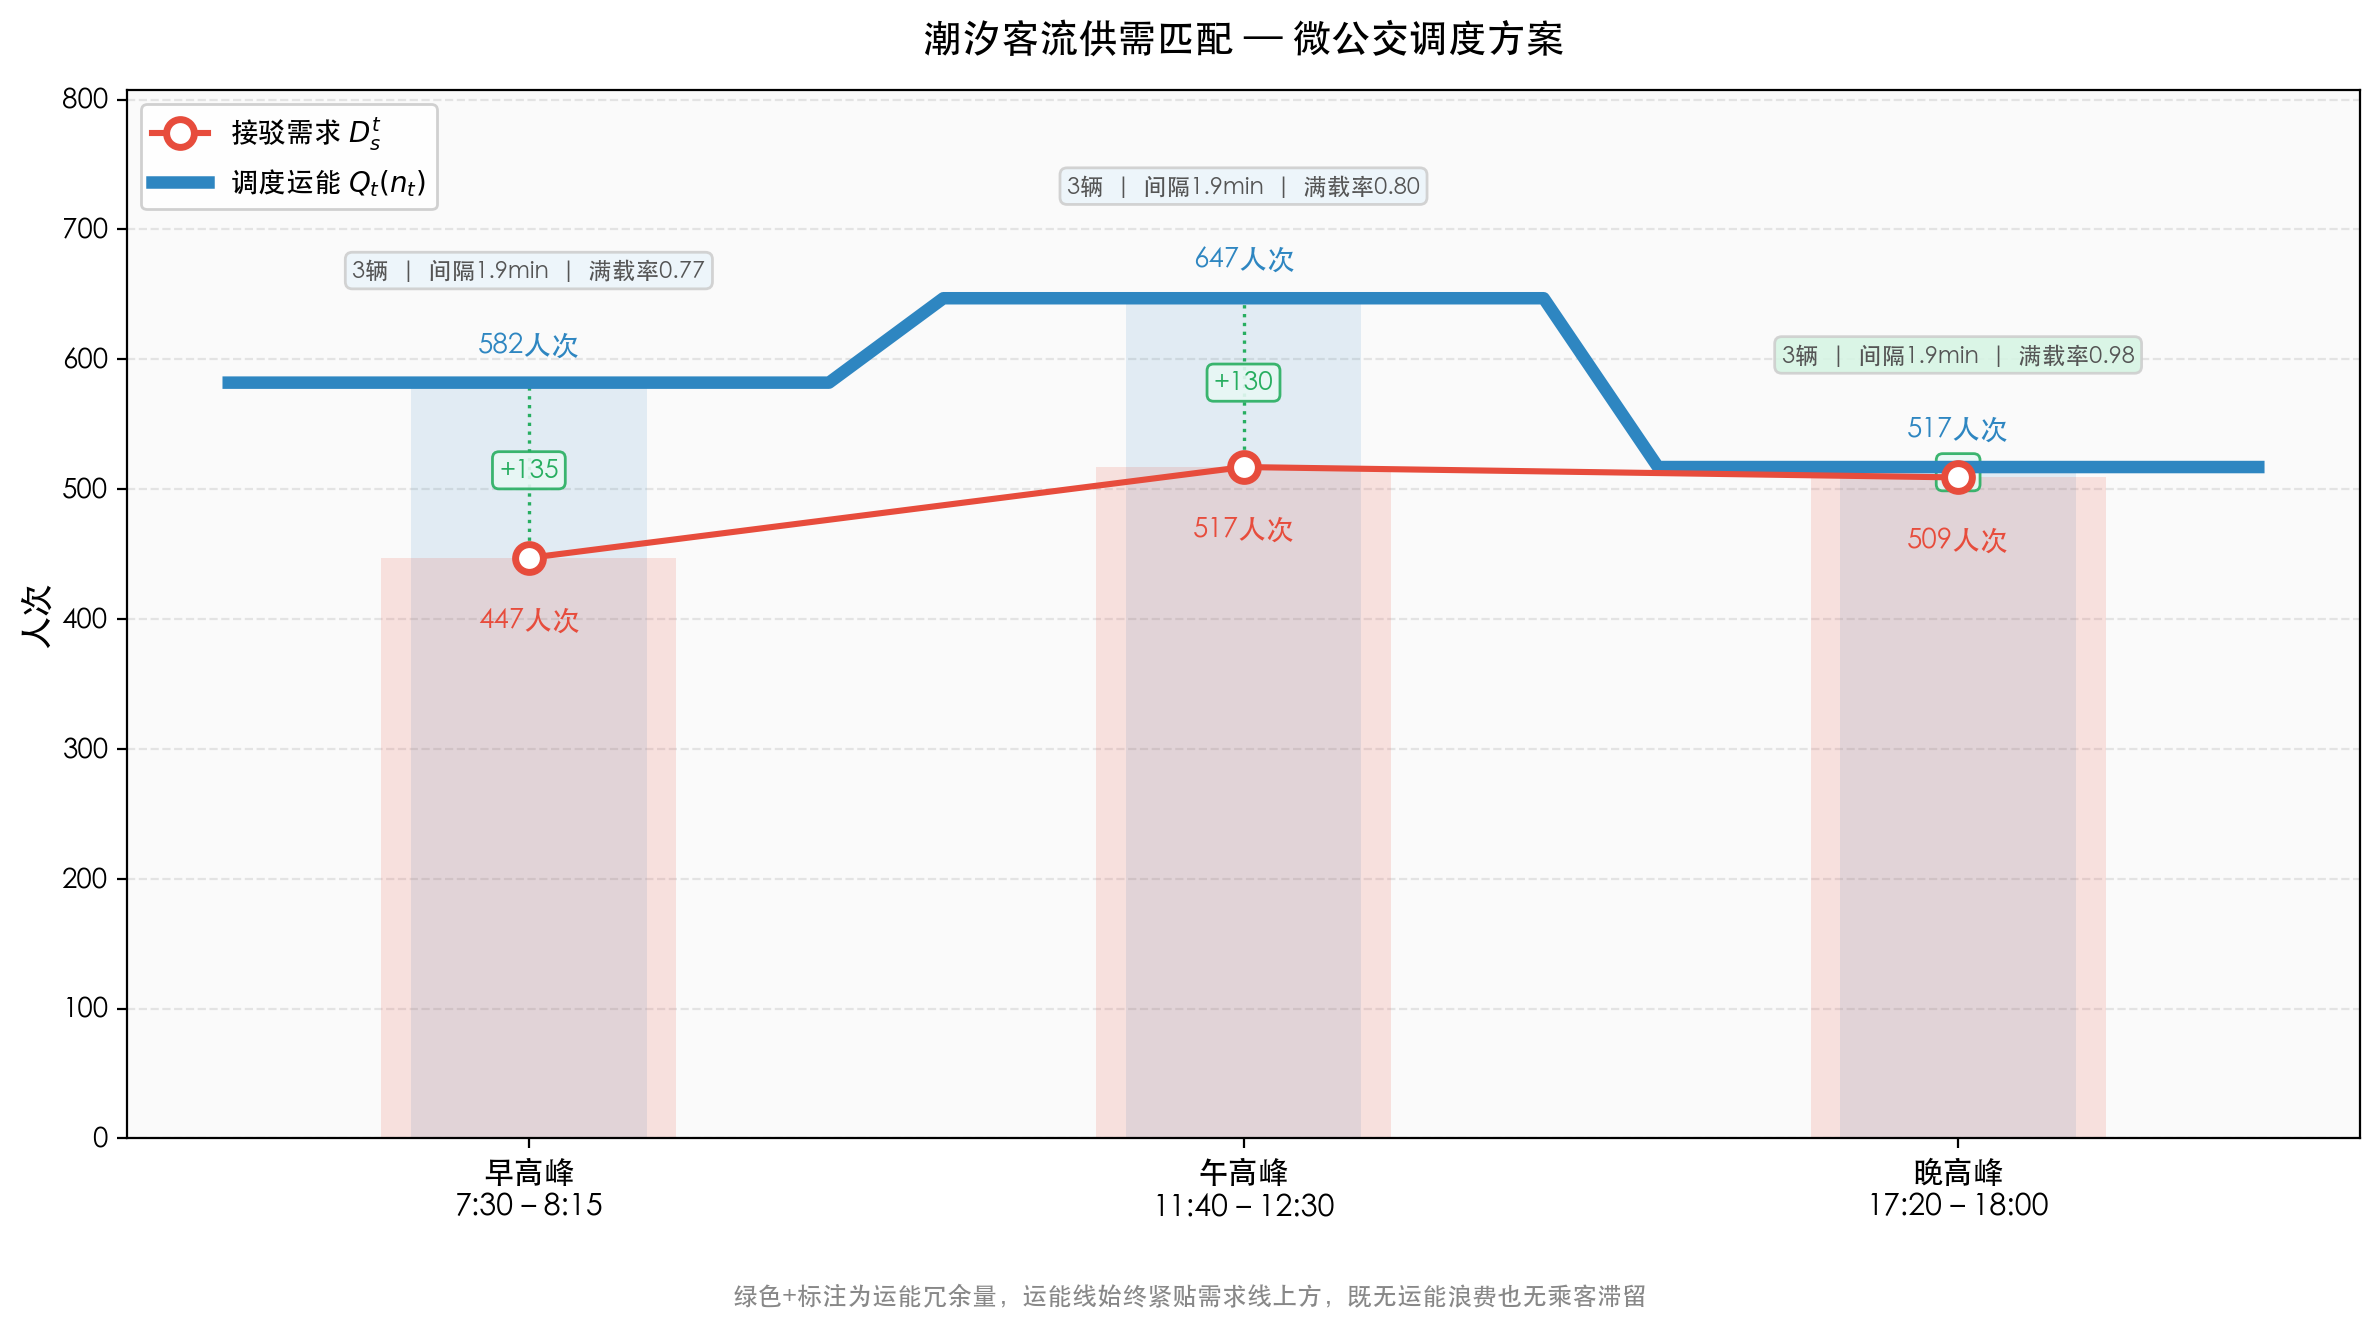
\includegraphics[width=0.65\linewidth]{figures/tidal_supply_demand.png}
\caption{潮汐客流供需匹配——微公交调度方案}
\label{fig:tidal_dispatch}
\end{figure}

\subsubsection{敏感性检验：基础替代率扰动}

为验证调度方案的鲁棒性，对核心参数基础绿色替代率 $\eta_{base}$ 在 $[0.05,0.25]$ 区间内以步长 $0.05$ 进行敏感性扫描。此时接驳需求退化为
\begin{equation}
D_s^t(\eta_{base})=\eta_{base}D_{bike}^t,\quad t\in\{\text{早},\text{午},\text{晚}\},
\end{equation}
代入调度模型重新求解各 $\eta_{base}$ 下的最优投放方案与成本构成，结果如表\ref{tab:sensitivity}所示。

\begin{table}[H]
\footnotesize
\centering
\caption{接驳车调度对基础替代率 $\eta_{base}$ 的敏感性}
\label{tab:sensitivity}
\begin{tabular}{ccccccc}
\toprule
$\eta_{base}$ & \textbf{早高峰 $n_t$} & \textbf{午高峰 $n_t$} & \textbf{晚高峰 $n_t$} & \textbf{总成本} & \textbf{满载率} & \textbf{冗余率} \\
\midrule
5\%  & 2 & 2 & 2 & 2886 & 0.64 & 36.2\% \\
10\% & 3 & 3 & 3 & 4149 & 0.85 & 15.0\% \\
15\% & 4 & 4 & 5 & 5593 & 0.88 & 11.7\% \\
20\% & 5 & 5 & 6 & 6713 & 0.95 & 4.5\% \\
25\% & 6 & 6 & 8 & 8126 & 0.96 & 4.0\% \\
\bottomrule
\end{tabular}
\end{table}

当 $\eta_{base}$ 扰动至 $25\%$ 时，运能平稳自适应（仅需调配备用车），满载率提升至0.96。说明模型能平滑应对需求激增，基于复合成本的调度机制非常稳健。

\newpage

\section{综合治理建议}

\subsection{问题重述}

问题四要求把前三问的模型结果转化成一页纸建议书，用通俗语言向管理层说明治理方案。
建议书需要回答校园最多能容纳多少非机动车，以及为什么要同步推进路网优化、停车治理和微公交接驳。
本问的重点不是重新建模，而是把前面得到的结论整理成可执行、可落地的管理建议。

\subsection{问题分析}

问题四主要是结果整合与表达转换：把问题一的路网优化结果、问题二的承载力上限、问题三的接驳方案统一整理成管理建议。
写作上采用“安全优先+总量控制+微公交替代”的思路，把定量结论转成学校可以直接执行的措施清单。

\subsection{模型假设}

作如下假设：
\begin{enumerate}
    \item 学校管理目标以安全优先为基本原则，在安全风险明显下降的前提下，可以接受小幅通行时间增加；
    \item 校园电动车治理既要考虑高峰同时运行需求，也要考虑实际保有量形成的长期存量压力；
    \item 微公交主要用于替代高峰私人电动车直达需求，不能单独吸收全部存量电动车；
\end{enumerate}

\subsection{符号说明}

\begin{table}[H]
\footnotesize
\centering
\caption{问题四主要符号说明}
\label{tab:symbols_q4}
\begin{tabular}{ccc}
\toprule
\textbf{符号} & \textbf{说明} & \textbf{单位} \\
\midrule
$N_{max}$ & 校园电动车安全环境承载力 & 辆 \\
$N_{stock}$ & 校园电动车实际保有量估计值 & 辆 \\
$\theta_{peak}$ & 高峰运行饱和度 & -- \\
$\theta_{stock}$ & 存量饱和度 & -- \\
$TTT$ & 全路网总行程时间 & 人$\cdot$s \\
$S$ & 人车冲突风险指标 & -- \\
$D_s^t$ & 时段 $t$ 微公交接驳需求 & 人次 \\
$Priority_k$ & 治理措施 $k$ 的综合优先级得分 & -- \\
\bottomrule
\end{tabular}
\end{table}

\subsection{模型的建立与求解}

\subsubsection{接驳效果评价与问题三结论}

将接驳车替代的电动车流量从原高峰OD中扣除，并重新进行交通分配，可得到微公交实施后的路网改善效果，如表\ref{tab:effect_result}所示。

\begin{table}[H]
\footnotesize
\centering
\caption{微公交接驳后的交通改善效果}
\label{tab:effect_result}
\begin{tabular}{cccccc}
\toprule
\textbf{时段} & \textbf{电动车削减率} & \textbf{TTT优化前} & \textbf{TTT优化后} & \textbf{TTT改善} & \textbf{冲突风险改善} \\
\midrule
早高峰 & 10.8\% & 2,557,530 & 2,488,595 & 2.7\% & 3.8\% \\
\bottomrule
\end{tabular}
\end{table}

\textbf{基准10\%替代率下，微公交使早高峰TTT下降2.7\%，$S$下降3.8\%，电动车出行削减10.8\%。}接驳车本身占用道路资源，改善幅度受替代率限制。\textbf{微公交的核心作用是减少私人电动车直达教学区、食堂和商业街的流量，分流核心区交通压力。}

\textbf{问题三推荐教学潮汐接驳线：桃园站—16号楼站—25号楼站—杏园站—桂苑站。早高峰和午高峰各3辆，晚高峰3辆。微公交与问题一的MinMax分流优化及问题二的核心区限停、总量控制共同构成综合治理方案。}

\subsubsection{前三问核心结果汇总}

根据前述模型测算：第一，MinMax增量分流算法在不改动道路的情况下，通过动态阻抗将瓶颈路段饱和度降低79.6\%，并输出了每对OD的具体分流路径，证明拥堵主因在于路径集中而非路网容量不足。第二，全校电动车安全承载力 $N_{max}=9414$ 的上限揭示出当前保有量（约 11000 辆）的存量饱和度达到 $1.168$，校园微交通长期面临超过 1586 辆的停放空间缺口，这是拥挤失序的本源。第三，以"桃园站—16号楼站—25号楼站—杏园站—桂苑站"为轴的潮汐接驳线只需投入三拨3辆校园公交，即可在高峰削减 10.8\% 的电动车需求，为校园路网减负。

\subsubsection{治理措施优先级评价框架}

设治理措施 $k$ 的综合优先级得分为
\begin{equation}
Priority_k=0.40Safety_k+0.35Capacity_k+0.25Feasibility_k,
\end{equation}
其中 $Safety_k$ 表示安全改善程度，$Capacity_k$ 表示容量缓解程度，$Feasibility_k$ 表示实施可行性。权重设置体现安全优先、兼顾容量和可操作性。

\begin{table}[H]
\footnotesize
\centering
\caption{校园微交通治理措施优先级排序}
\label{tab:priority_q4}
\begin{tabular}{ccccc}
\toprule
\textbf{治理措施} & \textbf{安全改善} & \textbf{容量缓解} & \textbf{可行性} & \textbf{优先级} \\
\midrule
清理消防通道、划定停车边界 & 高 & 高 & 高 & 第一优先 \\
16号楼、25号楼、商业街核心区限停 & 高 & 高 & 中 & 第一优先 \\
开通教学潮汐微公交线路 & 中 & 中 & 高 & 第二优先 \\
主干道人车隔离与分时限行 & 高 & 中 & 中 & 第二优先 \\
注册准入与存量车辆分期管控 & 高 & 高 & 中 & 长期推进 \\
外围集中停放与步行接驳引导 & 中 & 高 & 中 & 长期推进 \\
\bottomrule
\end{tabular}
\end{table}

由表\ref{tab:priority_q4}，第一优先为消防通道清理、停车边界划定和核心区限停；第二优先为教学潮汐微公交及主干道人车隔离、分时限行；长期推进注册准入与存量管控。

\subsubsection{面向管理层的一页纸建议书}

\begin{center}
{\heiti 关于浙师大金华校区校园“微交通”综合治理的建议书}
\end{center}

基于对校园道路、人车混行、电动车停放和微公交接驳系统的综合建模分析，我们建议学校采取"安全优先、总量控制、核心区限停、外围分流、公交替代"的综合治理策略，具体建议如下：

\textbf{明确承载上限，逐步控制电动车总量。}经测算，在严格保障消防与疏散通道的前提下，金华校区电动车安全承载力约为9414辆。当前校园实际保有量（超11000辆）已产生约1586辆的停放空间缺口。校园拥堵与乱停放的根源在于车辆存量已明显超出管理能力，建议学校以此承载力为参考，建立实名注册准入制度，逐步消化超载存量。

\textbf{实施路网动态分流引导，降低冲突风险。}模型评估显示，MinMax V/C增量分流算法在不改动路网结构的条件下，将瓶颈路段饱和度从1.249降至0.255（降幅79.6\%），全路网过饱和路段清零。建议基于模型输出的2284条最优分流路径，在关键路口设置导流标识，引导电动车流避开N4$\to$N14等拥堵瓶颈，实现车流的"自适应铺摊"。

\textbf{设立核心禁停区，引导外围停车。}16号楼、25号楼及商业街周边是目前校园停车矛盾最突出的区域。建议将这些区域设为核心限停区，严禁占用建筑出入口和主通道。同时，利用东区、西区新教学楼周边相对充足的容量作为缓冲，引导师生养成"外围停车、步行接驳进入核心区"的习惯。

\textbf{投放潮汐微公交，分担高峰直达车流。}建议开通连接主要生活区与核心教学区的微公交专线（如桃源站—16/25号楼—杏园—桂苑）。在早、中、晚高峰各投入3辆接驳车，即可满足高频连续发车需求。此举虽不能替代全部存量电动车，但能切实减少高峰期私人电动车直达核心区的规模，进一步缓解路网压力。

\textbf{分阶段稳步推进治理。}建议短期内以"清理消防通道、实施核心区限停"为抓手；中期配套微公交线路及候车设施；长期则落实电动车注册准入与分区管理。通过软硬结合，可在不大规模改造校园道路的前提下，切实提升校园交通的安全与有序。

\subsubsection{问题四结论}

\textbf{综合前三问结果：}路网优化的重点是降低冲突风险，电动车存量已超过安全承载力，微公交承担部分高峰替代和核心区分流功能。\textbf{管理建议：以9414辆为承载力参考上限，核心区限停和消防通道清理为近期重点，教学潮汐微公交为中期工具，注册准入和存量管控为长期手段。}

\section{模型评价与改进}

\subsection{模型优点}

\begin{enumerate}
\item 模型覆盖路网优化（UE）、承载力评估（静态/动态）和微公交规划（MCLP选址+调度），各问题间数据（路网、OD、容量）相互衔接。
\item 引入人车冲突风险指标$S$，将人车混行安全隐患量化为可优化的指标。
\item MinMax增量分流模型能输出每对OD的具体绕行路径和流量分配，为导流标识设置和出行推荐提供可直接落地的数据支撑。
\end{enumerate}

\subsection{模型缺点}

\begin{enumerate}
\item 引力模型替代实测OD数据，距离阶梯方式划分未考虑坡度、遮阳等因素。
\item BPR参数($\alpha=0.15,\beta=4.0$)为标准城市快速路取值，校园低速混行环境需实测标定。
\item 静态UE分配假设时段内需求均匀分布，低估了时段初的峰值拥堵效应。
\item 有效停车面积$A_i^{eff}$依赖暂估值，$\lambda_i$和原始候选面积需实地测量验证。
\item MCLP选址为静态模型，未考虑站点布局随学期规划或临时活动变化的动态调整需求。
\end{enumerate}

\subsection{模型推广}

本文模型可直接推广至具有类似教学--生活分区结构、以低速混行为主的其他大学校园或大型封闭园区，仅需替换路网数据和建筑容量参数。若引入实时导航App，UE假设需升级为随机用户均衡（SUE）或动态用户均衡（DUE）；若考虑电动车充电约束，OD模型需引入充电站节点；若治理涉及价格杠杆，决策变量需从$0$--$1$扩展为连续变量。

\begin{thebibliography}{9}
\bibitem{1} 王炜, 陈学武. 交通规划[M]. 3版. 北京: 人民交通出版社, 2017.
\bibitem{2} Bureau of Public Roads. Traffic Assignment Manual[R]. Washington, DC: U.S. Department of Commerce, 1964.
\bibitem{3} 王炜, 曲大义, 朱中. 城市交通网络综合平衡交通分配模型研究[J]. 东南大学学报(自然科学版), 2000, (01): 117-120.
\bibitem{4} Frank M, Wolfe P. An algorithm for quadratic programming[J]. Naval Research Logistics Quarterly, 1956, 3(1-2): 95-110.
\bibitem{5} 中华人民共和国住房和城乡建设部, 中华人民共和国国家质量监督检验检疫总局. GB\,50016--2014 建筑设计防火规范(2018年版)[S]. 北京: 中国计划出版社, 2018.
\bibitem{6} 住房和城乡建设部. 城市非机动车交通系统规划设计导则[S]. 北京: 中国建筑工业出版社, 2021.
\bibitem{7} Church R, ReVelle C. The maximal covering location problem[J]. Papers of the Regional Science Association, 1974, 32(1): 101-118.
\end{thebibliography}

\vspace{1em}
\noindent\textbf{说明：}本文参考文献的检索与整理工作由深度求索公司（DeepSeek v4 pro）辅助完成。

\newpage
\section*{附\quad 录}

\subsection*{附录目录}
\begin{enumerate}[leftmargin=3em]
  \item \textbf{附录A}：校园路网原始数据（\texttt{campus\_network\_with\_coords.txt}）
  \item \textbf{附录B}：步骤一：校园路网构建（\texttt{step1\_build\_graph.py}）
  \item \textbf{附录C}：步骤二：OD需求矩阵生成（\texttt{step2\_od\_matrix.py}）
  \item \textbf{附录D}：步骤三：多方式用户均衡分配（\texttt{step3\_ue\_fw.py}）
  \item \textbf{附录E}：步骤四：交通组织方案设计与对比（\texttt{step4\_scenarios.py}）
  \item \textbf{附录F}：步骤五：MinMax V/C增量分流（\texttt{step5\_k\_shortest.py}）
  \item \textbf{附录G}：步骤六：方案评价与报告输出（\texttt{step6\_evaluate.py}）
  \item \textbf{附录H}：步骤七：V/C热力图生成（\texttt{step7\_heatmap.py}）
  \item \textbf{附录I}：步骤八：功能区域划分（\texttt{step8\_zones.py}）
  \item \textbf{附录J}：步骤九：静态停车容量计算（\texttt{step9\_static.py}）
  \item \textbf{附录K}：步骤十：动态道路容量计算（\texttt{step10\_dynamic.py}）
  \item \textbf{附录L}：步骤十一：综合承载力求解（\texttt{step11\_solve.py}）
  \item \textbf{附录M}：步骤十二：问题三数据准备（\texttt{step12\_prepare.py}）
  \item \textbf{附录N}：步骤十三：候选站点构造与评价（\texttt{step13\_candidate\_stops.py}）
  \item \textbf{附录O}：步骤十四：MCLP最大覆盖选址（\texttt{step14\_coverage.py}）
  \item \textbf{附录P}：步骤十五：BPR阻抗线路规划（\texttt{step15\_routes.py}）
  \item \textbf{附录Q}：步骤十六：接驳需求识别与调度（\texttt{step16\_bus\_demand.py}）
  \item \textbf{附录R}：步骤十七：微公交效果评价（\texttt{step17\_effect.py}）
\end{enumerate}

\lstset{
  language=Python,
  basicstyle=\ttfamily\zihao{-5},
  columns=flexible,
  numbers=left,
  numberstyle=\tiny\color{gray},
  frame=single,
  breaklines=true,
  extendedchars=true,
  showstringspaces=false,
  aboveskip=0.5em,
  belowskip=0.5em,
}

\subsection*{附录A：校园路网原始数据 (\texttt{campus\_network\_with\_coords.txt})}
\lstset{language=, basicstyle=\ttfamily\zihao{-6}, numbers=none}
\lstinputlisting{code/campus_network_with_coords.txt}

\lstset{language=Python, basicstyle=\ttfamily\zihao{-5}, numbers=left}

\subsection*{附录B：步骤一：校园路网构建 (step1\_build\_graph.py)}
\lstinputlisting{code/step1_build_graph.py}

\subsection*{附录C：步骤二：OD需求矩阵生成 (step2\_od\_matrix.py)}
\lstinputlisting{code/step2_od_matrix.py}

\subsection*{附录D：步骤三：多方式用户均衡分配 (step3\_ue\_fw.py)}
\lstinputlisting{code/step3_ue_fw.py}

\subsection*{附录E：步骤四：交通组织方案设计与对比 (step4\_scenarios.py)}
\lstinputlisting{code/step4_scenarios.py}

\subsection*{附录F：步骤五：MinMax V/C增量分流 (step5\_k\_shortest.py)}
\lstinputlisting{code/step5_k_shortest.py}

\subsection*{附录G：步骤六：方案评价与报告输出 (step6\_evaluate.py)}
\lstinputlisting{code/step6_evaluate.py}

\subsection*{附录H：步骤七：V/C热力图生成 (step7\_heatmap.py)}
\lstinputlisting{code/step7_heatmap.py}

\subsection*{附录I：步骤八：功能区域划分 (step8\_zones.py)}
\lstinputlisting{code/step8_zones.py}

\subsection*{附录J：步骤九：静态停车容量计算 (step9\_static.py)}
\lstinputlisting{code/step9_static.py}

\subsection*{附录K：步骤十：动态道路容量计算 (step10\_dynamic.py)}
\lstinputlisting{code/step10_dynamic.py}

\subsection*{附录L：步骤十一：综合承载力求解 (step11\_solve.py)}
\lstinputlisting{code/step11_solve.py}

\subsection*{附录M：步骤十二：问题三数据准备 (step12\_prepare.py)}
\lstinputlisting{code/step12_prepare.py}

\subsection*{附录N：步骤十三：候选站点构造与评价 (step13\_candidate\_stops.py)}
\lstinputlisting{code/step13_candidate_stops.py}

\subsection*{附录O：步骤十四：MCLP最大覆盖选址 (step14\_coverage.py)}
\lstinputlisting{code/step14_coverage.py}

\subsection*{附录P：步骤十五：BPR阻抗线路规划 (step15\_routes.py)}
\lstinputlisting{code/step15_routes.py}

\subsection*{附录Q：步骤十六：接驳需求识别与调度 (step16\_bus\_demand.py)}
\lstinputlisting{code/step16_bus_demand.py}

\subsection*{附录R：步骤十七：微公交效果评价 (step17\_effect.py)}
\lstinputlisting{code/step17_effect.py}

\end{document}
